%%%%%%%%%%%%%%%%%%%%%%%%%%%%%%%%%%%%%%%%%
% Stylish Article
% LaTeX Template
% Version 2.0 (13/4/14)
%
% This template has been downloaded from:
% http://www.LaTeXTemplates.com
%
% Original author:
% Mathias Legrand (legrand.mathias@gmail.com)
%
% License:
% CC BY-NC-SA 3.0 (http://creativecommons.org/licenses/by-nc-sa/3.0/)
%
%%%%%%%%%%%%%%%%%%%%%%%%%%%%%%%%%%%%%%%%%

%----------------------------------------------------------------------------------------
%	PACKAGES AND OTHER DOCUMENT CONFIGURATIONS
%----------------------------------------------------------------------------------------

\documentclass[fleqn,10pt]{SelfArx} % Document font size and equations flushed left

\usepackage{lipsum} % Required to insert dummy text. To be removed otherwise
\usepackage{listings}
\usepackage{graphicx}
\graphicspath{Paper/images/}

%----------------------------------------------------------------------------------------
%	COLUMNS
%----------------------------------------------------------------------------------------

\setlength{\columnsep}{0.55cm} % Distance between the two columns of text
\setlength{\fboxrule}{0.75pt} % Width of the border around the abstract

%----------------------------------------------------------------------------------------
%	COLORS
%----------------------------------------------------------------------------------------

\definecolor{color1}{RGB}{0,0,90} % Color of the article title and sections
\definecolor{color2}{RGB}{0,20,20} % Color of the boxes behind the abstract and headings

%----------------------------------------------------------------------------------------
%	HYPERLINKS
%----------------------------------------------------------------------------------------

\usepackage{hyperref} % Required for hyperlinks
\hypersetup{hidelinks,colorlinks,breaklinks=true,urlcolor=color2,citecolor=color1,linkcolor=color1,bookmarksopen=false,pdftitle={Title},pdfauthor={Author}}

%----------------------------------------------------------------------------------------
%	ARTICLE INFORMATION
%----------------------------------------------------------------------------------------

\JournalInfo{Fuzzy Logic Expert System, December, 2019} % Journal information
\Archive{Go fuzzy or go home} % Additional notes (e.g. copyright, DOI, review/research article)

\PaperTitle{Fuzzy Logic Expert System} % Article title

\Authors{Robin Vonk, Michel Rummens} % Authors
% \textsuperscript{1}*
% \affiliation{\textsuperscript{1}\textit{Department of Biology, University of Examples, London, United Kingdom}} % Author affiliation
% \affiliation{\textsuperscript{2}\textit{Department of Chemistry, University of Examples, London, United Kingdom}} % Author affiliation
% \affiliation{*\textbf{Corresponding author}: john@smith.com} % Corresponding author

\Keywords{} % Keywords - if you don't want any simply remove all the text between the curly brackets
\newcommand{\keywordname}{Keywords} % Defines the keywords heading name

%----------------------------------------------------------------------------------------
%	ABSTRACT
%----------------------------------------------------------------------------------------

\Abstract{Report of our implementation of a fuzzy logic system, which is made with the python scikit-fuzzy library.}

%----------------------------------------------------------------------------------------

\begin{document}

\flushbottom % Makes all text pages the same height

\maketitle % Print the title and abstract box

\tableofcontents % Print the contents section

\thispagestyle{empty} % Removes page numbering from the first page

%----------------------------------------------------------------------------------------
%	ARTICLE CONTENTS
%----------------------------------------------------------------------------------------

\section*{Introduction} % The \section*{} command stops section numbering

\addcontentsline{toc}{section}{Introduction} % Adds this section to the table of contents
Hello children, today will take a look at the wonderful world of fuzzy logic. From the basics of a fuzzy control system, to some more advanced applications, we will give you a complete overview of why you should (not) use fuzzy logic. \\
%------------------------------------------------

\section{What is Fuzzy Logic}
Fuzzy Logic is an approach to variable processing that allows for multiple values to be processed through the same variable. Fuzzy logic attempts to solve problems with an open, imprecise spectrum of data that makes it possible to obtain an array of accurate conclusions. Fuzzy logic is designed to solve problems by considering all available information and making the best possible decision given the input.\\ \\
Fuzzy logic stems from the mathematical study of fuzzy concepts which also involves fuzzy sets of data. Mathematicians may use a variety of terms when referring to fuzzy concepts and fuzzy analysis. Broadly and comprehensively these terms are classified as fuzzy semantics.\\ \\
In practice, these constructs all allow for multiple values of the "true" condition. Instead of True being numerically equivalent to 1 and False being equivalent to 0 (or vice versa), the True condition could be any number of values less than one and greater than zero. This creates opportunity for algorithms to make decisions based on ranges of price data as opposed to one discreet data point.\\

% \begin{figure}[ht]\centering
% 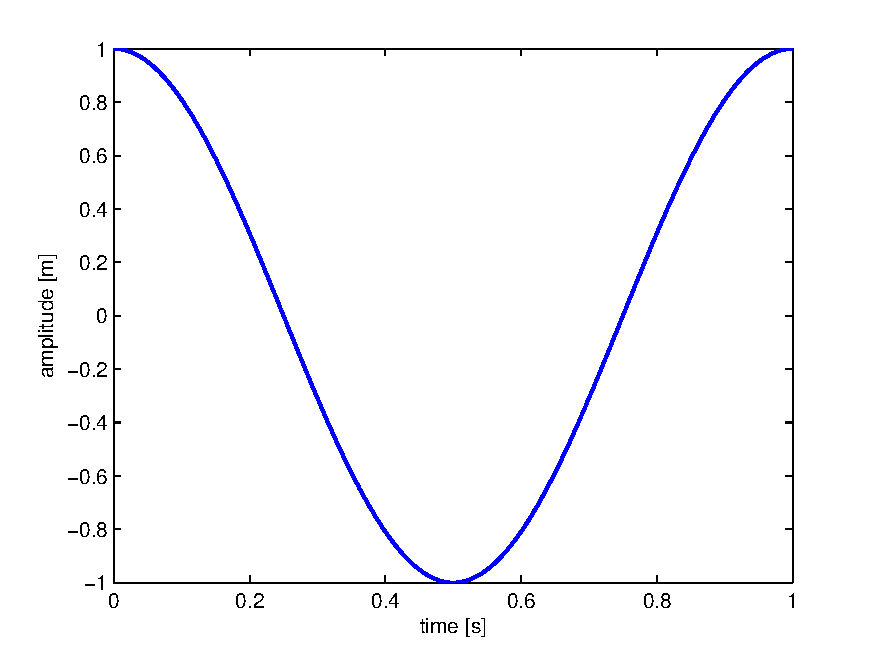
\includegraphics[width=\linewidth]{results}
% \caption{In-text Picture}
% \label{fig:results}
% \end{figure}

% Reference to Figure \ref{fig:results}.

%------------------------------------------------
\section{what is the scikit-fuzzy library}
The scikit-fuzzy library is a python library for creating fuzzy logic systems in a simple manner. It is part of the scikit library, which is a 'rather large' library for scientific purposes. It is often used to make a quick setup of a fuzzy system. However, making use of the library has it's constraints in usage, as with any library.
\subsection{Performance}
Under the hood, scikit-fuzzy makes use of NumPy library. NumPy-arrays are often used by scientific researchers because of it's possibilities to handle huge chunks of data, without having to worry about memory management. The downside of the easy usage is the performance. NumPy-arrays are stored directly into your storage, instead of in memory. This eliminates the need of worrying about maximum size of data-types, but does cost performance. Storage devices (HDD/SSD) often respond way slower than memory (RAM).\\ \\
So if you are looking to build a fast responding fuzzy logic system, your best bet would probably be writing it in pure C / C++.


\subsection{Used fuzzy algorithms}
The scikit fuzzy library uses a modular design for its algorithms. This means that it has separate packages for each algorithm, which could be extended with different approaches of the algorithm. It has the following packages for algorithms:
\begin{itemize}
    \item cluster: A package containing the c-means algorithm. This algorithm manages the format the data is stored in. 
    \item control: A package providing control over the other algorithms.
    \item defuzzify: A package containing algorithms for defuzzifying a cluster (getting a crispy value).
    \item filters: A package containing possible filters for a cluster.
    \item fuzzymath: A package containing algorithms for doing mathematical operations on fuzzy clusters.
    \item image: A package containing algorithm to convert a cluster to an image.
    \item intervals: A package containing algorithms for calculations between membership functions.
    \item membership: A package containing algorithms for generating membership functions. 
\end{itemize}
The algorithms used for clustering the data (the fuzzy c-mean clustering algorithm) is completely written in Python. This is a disadvantage, because of the speed of python with big data sets, compared to other programming languages. \cite{Benchmark} What is also confirmed by the creators of the scikit fuzzy library. \cite{SciPy} This means that the scikit library should be slower than other libraries for Python which use Cython of C code for the calculations. We have not tested this however, so it is only an expectation.\\ \\

The modular approach for the algorithms is very useful. Separating the different parts of the application makes it a lot easier to understand what happens in the different parts of the code. This allowed the developers to create a logical documentation structure in the code, from very abstract in the application to very specific working of functions. For example, in the membership package they explain in global what a membership function does and refer to the possible algorithms to use. In each of these algorithms they explain the specific implementation of that membership algorithm. This way they create a good and clear hierarchical tree for the documentation. \\  
The modular approach also allows you to change the system to your own needs. For example, you could add your own algorithm based on C code to improve the speed of the system.


\section{How to use the scikit-fuzzy library}

\subsection{Installation}
To install the scikit-fuzzy library for python on your system, simply use: 
\begin{lstlisting}[language=Python]
pip install scikit-fuzzy
\end{lstlisting}

\subsection{Creating the inputs/outputs}
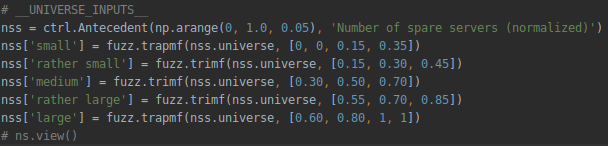
\includegraphics[width=9cm]{Paper/images/universe.png}
As can be seen (sort of) in the picture above, creating an input/output can be done very simply be just a few lines of code. By creating an input/output, you define a set of value ranges - also known as the universe - which make sense for the system you are constructing.
Inputs are denoted as Antecedent and outputs as Consequent.
\subsection{Creating a rule base}
Once the inputs and outputs are created, the next step is to define a set of rules which make sense to your system, based on the inputs and outputs.
In our example, we have the inputs 'number of spare parts (normalized) (nss)', 'Mean delay (normalized) (md)' and 'Repair utilisation factor (ruf)'. The only output in our system is 'Number of spare parts (normalized) (nsp)', but there could be multiple outputs. 
Our system calculates the number of spare parts (normalized), based on the inputs. A few rules of our rule base are:

\begin{itemize}
    \item ctrl.Rule(ruf['low'], nsp['small'])
    \item ctrl.Rule(md['small'] \& nss['large'], nsp['small'])
\end{itemize}
The first rule states that if the ruf is low, the nsp should be small.\\
The second rule states that if the md is small AND the nss is large, the nsp should be small.\\
Our rule base consists of 21 rules and covers every scenario based on our inputs and outputs. 


\subsection{Using the system}
Once all rules are created, you can set up the system, based on the inputs/outputs and the rule base you have created. You could also very easily create a slightly different system based on a subset of rules and inputs/outputs, but for now let's continue with the system as described earlier.
For creating the system and reading it's output, there are a few steps to be taken in the following order:

\begin{itemize}
    \item Create the control system based on the rule base:\\
    spare\_parts\_ctrl = ctrl.ControlSystem(rules1)
    \item Create a control system simulation based on the control system:\\
    spare\_parts = ctrl.ControlSystemSimulation(spare\_parts\_ctrl)
    \item Feed the input values yo the control system simulation:\\
    spare\_parts.input['Number of spare servers (normalized)'] = 0.2\\
    spare\_parts.input['Repair utilisation factor'] = 0.2\\
    spare\_parts.input['Mean delay (normalized)'] = 0.0
    \item Start the computation\\
    spare\_parts.compute()
    \item Read the output\\
    spare\_parts.output['Number of spare parts (normalized)']
    \item View the graph generated for the output (optional)\\
    nsp.view(sim=spare\_parts)
\end{itemize}
The library is written in a very modular way, if you would like to use a different rule base for your system, simply replace the rule base with a different one. The same goes for the inputs/outputs and even some algorithms used. Using it as such does require some splitting in rule bases and combinations of inputs/outputs.

\subsection{Community questions}
Jan Derriks heard we were writing this report, and asked us to research whether scikit-fuzzy is save to use within a pepper-robot. 

\subsection{Safety of the scikit-fuzzy library}
Regarding hacker-proof safety, we don't think this is an issue. The only thing that could be an issue is the entry point of your program. Make sure users are not able to execute commands by entering certain commands into your inputs.\\ \\
The other aspect we could think of is safety in usage. The library is very safe to use because it makes use of the NumPy library (arrays). In other programming languages and libraries calculating big numbers (data), you will need to worry about it's size and whether the output is really close enough to what you expect it to be. NumPy takes away this worry - at some cost of performance - but ensures safety in usage to some degree.

\subsection{Demo}
An example system in python can be found on the Github page: \\
\url{https://github.com/obin1000/Fuzzy_Logic_Expert_System}

\section{Pros and cons of using the scikit-fuzzy library}

\subsection{Pros}
\begin{itemize}
    \item Easy to use (safe in usage)
    \item Quick to use
    \item Modular design for simple customization
    \item Well documented
\end{itemize}
\subsection{Cons}
\begin{itemize}
    \item Bad performance (Slow execution time)
\end{itemize}

%------------------------------------------------
% \phantomsection
% \section*{Acknowledgments} % The \section*{} command stops section numbering

% \addcontentsline{toc}{section}{Acknowledgments} % Adds this section to the table of contents

% So long and thanks for all the fish \cite{Figueredo:2009dg}.

%----------------------------------------------------------------------------------------
%	REFERENCE LIST
%----------------------------------------------------------------------------------------
\phantomsection
\bibliographystyle{unsrt}
\bibliography{References}

%----------------------------------------------------------------------------------------

\end{document}